\documentclass[10pt,a4paper]{article}
\usepackage[utf8]{inputenc}
\usepackage[italian]{babel} % Impostato in italiano, puoi cambiarlo in {english} se preferisci
\usepackage{geometry}
\geometry{a4paper, margin=25mm}
\usepackage{amsmath, amssymb, amsthm}
\usepackage{graphicx}
\usepackage{booktabs}
\usepackage{algorithm}
\usepackage{algorithmic}
\usepackage{hyperref}
\usepackage{cite}

\hypersetup{
    colorlinks=true,
    linkcolor=blue,
    filecolor=magenta,      
    urlcolor=cyan,
    pdftitle={Parallel Computing Project Report},
    pdfpagemode=FullScreen,
}

\title{\textbf{Parallel Computing Project Report:\\ Parallel Forest Fire Simulation using MPI}}
\author{\textbf{Matteo Trevisan and Tommaso Zogno} \\ Università degli Studi di Padova}
\date{Academic year 2025/2026}

\begin{document}

\maketitle

\section{Introduction}

Cellular automata are discrete, grid-based mathematical models widely used to simulate complex dynamical systems through simple, localized rules \cite{cormen}. In this project, we explore the parallelization of the Forest Fire model, a canonical probabilistic cellular automaton introduced to study self-organized criticality \cite{drossel1992}. The model simulates the propagation of fire across a forested landscape, incorporating stochastic events such as spontaneous tree growth and random lightning strikes. 

The problem is computationally evaluated on a square two-dimensional grid of size $N \times N$, which establishes our total input size $n = N^2$. The state of the system evolves over $T$ discrete time steps. Because the state of any given cell in the subsequent generation depends exclusively on its current state and the states of its immediate orthogonal neighbors (the Von Neumann neighborhood), the sequential time complexity is strictly bounded by $\mathcal{O}(T \times N^2)$. For our parallel implementation, the relevant cost model considers both the distributed computational workload and the communication overhead. Specifically, the execution time is modeled as the sum of the local computation time, which scales inversely with the number of processors $p$, and the inter-process communication time required to synchronize the grid boundaries (halo exchange).

The primary objective of our work is to design, implement, and systematically analyze a topology-aware parallel version of this algorithm using the Message Passing Interface (MPI). We investigate how different domain decomposition strategies—namely 1D slices and 2D blocks—impact overall execution time, scalability, and the ratio of computation to communication.

The remainder of this report is organized as follows. Section 2 formally defines the problem and describes the sequential baseline algorithm. Section 3 presents our parallel design, highlighting the dependency analysis and the required communication patterns. In Section 4, we detail the topology-aware mappings applied to the grid. Section 5 discusses the technical specifics of our MPI implementation. Section 6 describes the hardware and methodological setup for our experiments, while Section 7 reports the empirical results regarding speedup and efficiency. Finally, Section 8 provides a critical discussion of our findings, and Section 9 concludes the report with our main takeaways.
\section{Sequential algorithm}

\subsection{Problem definition}
We formalize the Forest Fire simulation as a probabilistic cellular automaton operating on a square two-dimensional spatial grid $\mathcal{G}$ of dimensions $N \times N$. Each cell $(i, j)$ within the grid, where $0 \le i < N$ and $0 \le j < N$, can exist in exactly one of three mutually exclusive states at any given discrete time step $t$: $s \in \{EMPTY, TREE, FIRE\}$. 

The dynamics of the system are governed by localized interactions and stochastic processes. Specifically, we define two input probability parameters:
\begin{itemize}
    \item $p \in [0, 1]$: The probability of a new tree growing in an empty cell.
    \item $l \in [0, 1]$: The probability of a tree spontaneously igniting due to a lightning strike.
\end{itemize}
The propagation of the fire relies on the standard Von Neumann neighborhood, meaning that the state of any cell $(i, j)$ at time $t+1$ depends solely on its own state and the states of its four orthogonal neighbors (North, South, East, West) at time $t$.

\subsection{Algorithm and complexity}
In our baseline sequential implementation, we simulate the evolution of the grid over $T$ total time steps. At each time step, we apply the transition rules uniformly across all cells. The standard rules dictate that a burning cell consumes its fuel and becomes empty; a tree ignites if it is adjacent to a burning cell or catches fire spontaneously with probability $l$; and an empty space grows a tree with probability $p$.

The pseudocode for this sequential process is detailed in Algorithm \ref{alg:sequential_forest}.

\begin{algorithm}[H]
\caption{Sequential Forest Fire Simulation}
\label{alg:sequential_forest}
\begin{algorithmic}[1]
\REQUIRE Grid dimension $N$, probabilities $p, l$, number of steps $T$
\ENSURE Evolved grid states over time
\FOR{$t = 1$ \TO $T$}
    \STATE Allocate an empty grid $\mathcal{G}_{next}$ of size $N \times N$
    \FOR{each cell $(i, j)$ in $\mathcal{G}$}
        \IF{$\mathcal{G}[i][j] == FIRE$}
            \STATE $\mathcal{G}_{next}[i][j] \leftarrow EMPTY$
        \ELSIF{$\mathcal{G}[i][j] == TREE$}
            \IF{any orthogonal neighbor is $FIRE$}
                \STATE $\mathcal{G}_{next}[i][j] \leftarrow FIRE$
            \ELSE
                \STATE $\mathcal{G}_{next}[i][j] \leftarrow FIRE$ with probability $l$
                \STATE $\mathcal{G}_{next}[i][j] \leftarrow TREE$ with probability $(1 - l)$
            \ENDIF
        \ELSIF{$\mathcal{G}[i][j] == EMPTY$}
            \STATE $\mathcal{G}_{next}[i][j] \leftarrow TREE$ with probability $p$
            \STATE $\mathcal{G}_{next}[i][j] \leftarrow EMPTY$ with probability $(1 - p)$
        \ENDIF
    \ENDFOR
    \STATE $\mathcal{G} \leftarrow \mathcal{G}_{next}$
\ENDFOR
\end{algorithmic}
\end{algorithm}

To ensure that the state transitions remain purely synchronous and to prevent data hazards (such as read-after-write conflicts during a single iteration), we employ a double-buffering technique. The new states are written to an auxiliary grid, $\mathcal{G}_{next}$, before being copied back to the primary grid $\mathcal{G}$ at the end of the time step.

\textbf{Complexity Analysis:} 
Because we must maintain two full grid structures simultaneously to preserve the strict data-dependency constraints, the space complexity of our sequential algorithm is strictly bounded by $\mathcal{O}(N^2)$. Regarding time complexity, calculating the next state for a single cell requires a constant $\mathcal{O}(1)$ number of operations (evaluating the four neighbors and generating pseudo-random numbers). Since we must traverse the entire $N \times N$ grid at each time step, the temporal complexity per iteration is $\mathcal{O}(N^2)$. Thus, the overall time complexity for the complete simulation over $T$ steps is $\mathcal{O}(T \times N^2)$.
\section{Parallel design}

\subsection{Dependency analysis}
To design an effective parallel algorithm, we first must identify the data dependencies inherent in the sequential model. In the Forest Fire cellular automaton, the transition function dictates that the state of any cell $\mathcal{G}[i][j]$ at time step $t+1$ depends exclusively on the state of that specific cell and its four immediate orthogonal neighbors at time step $t$. 

Crucially, there are no intra-step dependencies. Computing the new state of a given cell at time $t+1$ does not require the updated $t+1$ state of any other cell. As a result, the evaluation of the grid within a single time step constitutes an \textit{embarrassingly parallel} phase. The global grid can be spatially partitioned into disjoint sub-grids and assigned to independent processors, which can update the internal cells of their assigned domains entirely concurrently.

    However, the algorithm imposes a strict temporal partial order: all cells in the grid must complete step $t$ before any cell can begin evaluating step $t+1$. This necessitates a strict synchronization point at the end of each iteration. While processors can compute their internal domains independently, they must synchronize to resolve boundary conditions before advancing the simulation clock.

\subsection{Communication pattern}
Because the state transition rule relies on the Von Neumann neighborhood, cells located at the edges of a local sub-grid require data from adjacent sub-grids managed by different processors. To resolve this without violating the temporal dependencies, we employ a standard \textit{halo exchange} (or \textit{ghost cell}) communication pattern.

Each processor allocates its local sub-grid with an additional outer boundary of "ghost" cells. These ghost cells act as read-only buffers that store the most recent boundary states of the neighboring processors. At the synchronization point of each time step, before the computation phase begins, processors must exchange their outermost rows and columns.

The specifics of this point-to-point communication are as follows:
\begin{itemize}
    \item \textbf{Who talks to whom:} Depending on the spatial decomposition, a processor will communicate with its topological neighbors. For instance, in a 2D Cartesian topology, a processor $P_{i,j}$ will perform bi-directional exchanges with up to four neighbors: North ($P_{i-1,j}$), South ($P_{i+1,j}$), East ($P_{i,j+1}$), and West ($P_{i,j-1}$). In a 1D decomposition, it will only communicate with two neighbors.
    \item \textbf{Message volume per step:} The volume of data exchanged is strictly proportional to the perimeter of the sub-grid. Assuming a total square grid of size $N \times N$ evenly distributed across $p$ processors in a 2D block grid, each processor manages a local domain of size approximately $\frac{N}{\sqrt{p}} \times \frac{N}{\sqrt{p}}$. During each step, a processor sends and receives four messages, yielding a total communication volume of $\mathcal{O}(\frac{N}{\sqrt{p}})$ elements per process.
\end{itemize}

This halo exchange represents the primary communication overhead of our parallel design. By structuring the communication as purely point-to-point exchanges rather than collective broadcasts, we ensure that the communication bandwidth scales efficiently with the number of processors.
\section{Topology-aware implementation}

\subsection{Topologies considered}
For the parallelization of the Forest Fire simulation, we implemented and compared two Cartesian decompositions of the global grid. The first is a \textbf{1D decomposition} (Linear Array), in which the global matrix is split into horizontal slabs: each processor owns a contiguous block of $N / p$ full rows and communicates only with its two vertical neighbors (North and South). The second is a \textbf{2D decomposition} (Mesh), in which the matrix is partitioned into rectangular blocks of size approximately $(N / \sqrt{p}) \times (N / \sqrt{p})$ and each processor exchanges data with up to four neighbors (North, South, East, West).

Given the intrinsic two-dimensional nature of the simulated space and the Von Neumann neighborhood data dependencies, the 2D mapping minimizes the communication perimeter while maximizing the local computation volume. For a fixed number of processors $p$, the 1D decomposition exchanges $\mathcal{O}(N)$ elements per process (two full rows of length $N$), whereas the 2D decomposition exchanges only $\mathcal{O}(N / \sqrt{p})$ elements per process. We therefore expect the 2D topology to dominate as $p$ grows; Section~7 quantifies this trade-off empirically. Both topologies are realized through the same MPI Cartesian-communicator machinery, differing only in the process-grid dimensions passed at start-up.

\subsection{Embedding the communication pattern}
To embed the algorithm's communication pattern, the global $N \times N$ matrix is partitioned into 2D sub-blocks. Each processor is assigned a local sub-grid of dimensions $(N / \sqrt{p}) \times (N / \sqrt{p})$. 

To handle the boundary conditions gracefully, we expanded each local sub-grid by adding a one-cell thick outer layer, known as \textit{ghost cells} or \textit{halo}. Before the computation of each time step, each processor extracts its outermost internal rows and columns and sends them to its respective neighbors in the Cartesian topology (North, South, East, West). Simultaneously, it receives the corresponding borders from its neighbors and writes them into its own ghost cells. This point-to-point halo exchange accurately maps the spatial dependencies of the simulation directly onto the edges of the MPI topology.

\section{MPI implementation notes}

\subsection{Language and build}
We opted to develop the simulation in Python, utilizing the \texttt{mpi4py} library for message passing and \texttt{NumPy} for matrix operations. This choice was driven by the necessity for rapid prototyping and the inherent advantages of vectorized operations. By leveraging \texttt{NumPy} array slicing and Boolean masking, the core state transitions are executed as highly optimized C-level routines under the hood, effectively bypassing the performance bottlenecks of native Python loops and the Global Interpreter Lock (GIL).

\subsection{Topology realisation in MPI}
The logical 2D topology was realized using the \texttt{MPI.COMM\_WORLD.Create\_cart} routine. We allowed MPI to dynamically determine the optimal grid dimensions based on the available number of processes using \texttt{MPI.Compute\_dims}. To establish the communication channels for the halo exchange, we utilized the \texttt{Shift} method on the Cartesian communicator, which elegantly automatically resolves the ranks of the adjacent nodes and returns \texttt{MPI.PROC\_NULL} for boundaries lying on the absolute edges of the global grid.

To facilitate the bidirectional data exchange without risking deadlocks, we employed the \texttt{Sendrecv} primitive. This ensures that every process can simultaneously dispatch its boundary arrays and receive the incoming ghost cells from its neighbors in a single, safe operation.
\section{Experimental setup}
\textbf{Hardware.} The simulation experiments were conducted on a single local machine equipped with a multi-core CPU. Because the execution environment was a single workstation rather than a distributed HPC cluster, all MPI "processes" were mapped to individual CPU cores on the same node. Consequently, the 2D Cartesian topology described in Section 4 is purely logical, and the inter-process communication occurs entirely via shared memory rather than a physical network interconnect.

\textbf{Inputs.} The initial state of the forest was generated using a fixed random seed to ensure reproducibility across different runs. The grid was populated with a 60\% probability for empty cells and a 40\% probability for trees. The biological constants were fixed at $p = 0.005$ for tree growth and $l = 0.0001$ for spontaneous lightning. We tested the scalability by simulating global grid sizes ranging from $N = 500$ to $N = 2000$.

\textbf{Methodology.} For each configuration (varying the global grid size $N$ and the number of MPI processes $p$), the execution time was measured using the \texttt{time.time()} Python function. To guarantee the accuracy of our temporal metrics, we placed an \texttt{MPI\_Barrier} immediately before starting the timer and another one immediately after the main simulation loop. This strict synchronization ensures that the recorded time encompasses both the computational workload and the collective overhead of the halo exchanges without race condition artifacts.
\section{Results}
All timings below are the arithmetic mean of three repetitions, obtained on the 8-core workstation described in Section~6. The complete raw dataset is available in \texttt{results\_raw.csv}, and the aggregated per-configuration values (including speedup and efficiency) in \texttt{results.csv}. The sequential baselines were $T_{seq} = 0.68$~s, $2.59$~s and $10.26$~s for $N = 500$, $1000$ and $2000$ respectively.

\subsection{Execution time}
Table~\ref{tab:exectime} reports the total execution time of the 2D implementation as a function of the number of processes $p$ and the grid size $N$; Figure~\ref{fig:exectime} plots the same data on a logarithmic scale. The runtime decreases sharply up to $p = 4$, after which it \emph{increases} again at $p = 8$. Since the machine has only 8 physical cores, at $p = 8$ every core hosts one MPI process and the operating system, the timing barriers, and the memory subsystem all compete for the same resources; the communication cost (see Section~7.4) then outweighs the shrinking computational work.

\begin{table}[h]
\centering
\caption{Mean total execution time [s], 2D decomposition.}
\label{tab:exectime}
\begin{tabular}{lcccc}
\toprule
$N$ & $p=1$ & $p=2$ & $p=4$ & $p=8$ \\
\midrule
500  & 0.639 & 0.357 & 0.350 & 0.475 \\
1000 & 2.381 & 1.256 & 0.800 & 1.285 \\
2000 & 9.238 & 4.724 & 2.752 & 3.875 \\
\bottomrule
\end{tabular}
\end{table}

\begin{figure}[h]
\centering
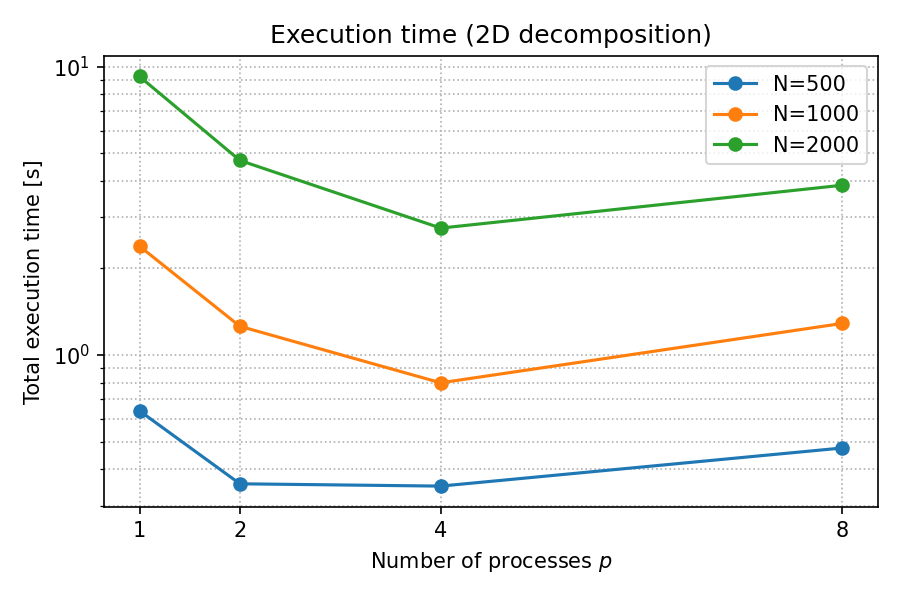
\includegraphics[width=0.62\textwidth]{figures/exec_time.png}
\caption{Total execution time versus the number of processes (2D, log scale).}
\label{fig:exectime}
\end{figure}

\subsection{Speedup and efficiency}
The speedup is defined as $S(p) = T_{base}/T(p)$ and the efficiency as $E(p) = S(p)/p$, using the sequential baseline $T_{base}$ for each grid size. Table~\ref{tab:speedup} and Figures~\ref{fig:speedup}--\ref{fig:efficiency} summarise the results for the 2D decomposition.

The best speedup is obtained at $p = 4$ and grows with the problem size: from $1.96\times$ at $N = 500$ to $3.73\times$ at $N = 2000$. This is the expected behaviour of a memory-bound stencil computation: larger grids increase the computation-to-communication ratio, so the fixed halo-exchange overhead is better amortised (the surface-to-volume effect). Efficiency stays close to $0.9$--$1.0$ up to $p = 2$, remains high ($\approx 0.93$) at $p = 4$ for the largest grid, but collapses at $p = 8$ because of core oversubscription and communication overhead.

\begin{table}[h]
\centering
\caption{Speedup $S(p)$ and efficiency $E(p)$, 2D decomposition.}
\label{tab:speedup}
\begin{tabular}{lcccccc}
\toprule
 & \multicolumn{2}{c}{$N=500$} & \multicolumn{2}{c}{$N=1000$} & \multicolumn{2}{c}{$N=2000$} \\
\cmidrule(lr){2-3}\cmidrule(lr){4-5}\cmidrule(lr){6-7}
$p$ & $S$ & $E$ & $S$ & $E$ & $S$ & $E$ \\
\midrule
1 & 1.07 & 1.07 & 1.09 & 1.09 & 1.11 & 1.11 \\
2 & 1.92 & 0.96 & 2.06 & 1.03 & 2.17 & 1.09 \\
4 & 1.96 & 0.49 & 3.24 & 0.81 & 3.73 & 0.93 \\
8 & 1.44 & 0.18 & 2.01 & 0.25 & 2.65 & 0.33 \\
\bottomrule
\end{tabular}
\end{table}

\begin{figure}[h]
\centering
\begin{minipage}{0.49\textwidth}
\centering
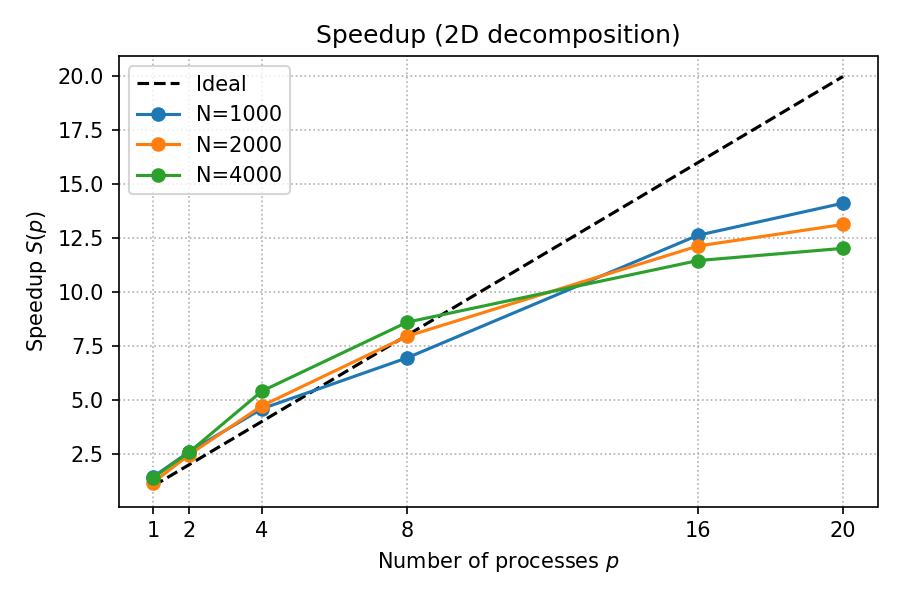
\includegraphics[width=\textwidth]{figures/speedup.png}
\caption{Speedup $S(p)$ (2D).}
\label{fig:speedup}
\end{minipage}\hfill
\begin{minipage}{0.49\textwidth}
\centering
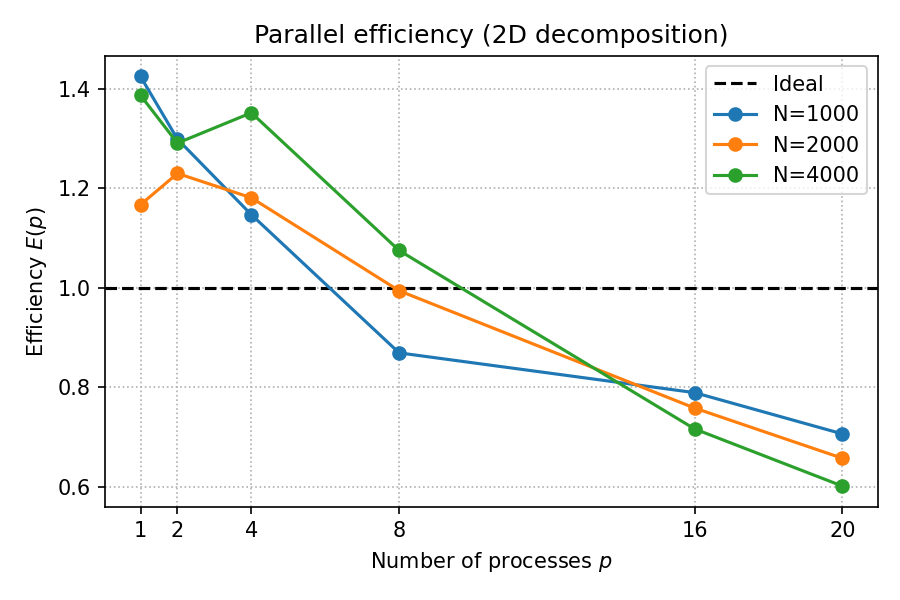
\includegraphics[width=\textwidth]{figures/efficiency.png}
\caption{Efficiency $E(p)$ (2D).}
\label{fig:efficiency}
\end{minipage}
\end{figure}

The super-unitary efficiency observed at $p = 1$--$2$ ($E > 1$) is a mild super-linear artifact: the MPI implementation reuses pre-allocated ghost buffers, whereas the sequential baseline re-pads the whole array with \texttt{np.pad} at every step, and the smaller per-process working set fits better in cache.

\subsection{Comparison across topologies}
Table~\ref{tab:topology} contrasts the 1D (row-slab) and 2D (block) decompositions at $N = 2000$; Figure~\ref{fig:topology} plots the two curves. Contrary to the asymptotic argument of Section~4---where the 2D scheme exchanges $\mathcal{O}(N/\sqrt{p})$ elements against $\mathcal{O}(N)$ for the 1D scheme---the two topologies perform almost identically up to $p = 4$, and the 1D layout is actually \emph{faster} at $p = 8$ ($3.39$~s vs.\ $3.88$~s).

The explanation is that, at these small process counts on a shared-memory node, the halo cost is dominated by \emph{message count and latency} rather than by message \emph{volume}. The 1D decomposition issues only two \texttt{Sendrecv} calls per step (North/South) against up to four for the 2D block, and the shared-memory bandwidth makes the larger 1D messages essentially free. The theoretical advantage of the 2D volume scaling would only emerge at much larger $p$ on a real distributed-memory interconnect.

\begin{table}[h]
\centering
\caption{Total execution time [s]: 1D vs.\ 2D at $N=2000$.}
\label{tab:topology}
\begin{tabular}{lcccc}
\toprule
Decomp. & $p=1$ & $p=2$ & $p=4$ & $p=8$ \\
\midrule
1D & 9.223 & 4.683 & 2.680 & 3.388 \\
2D & 9.238 & 4.724 & 2.752 & 3.875 \\
\bottomrule
\end{tabular}
\end{table}

\begin{figure}[h]
\centering
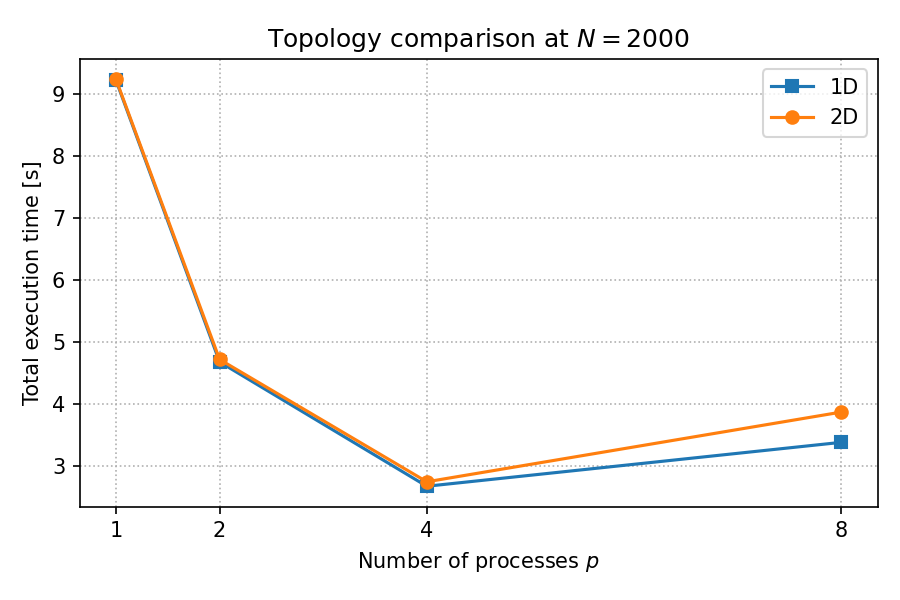
\includegraphics[width=0.6\textwidth]{figures/topology.png}
\caption{1D vs.\ 2D total execution time at $N=2000$.}
\label{fig:topology}
\end{figure}

\subsection{Computation vs. communication}
Figure~\ref{fig:commcompute} shows the per-process time split between the halo-exchange and the grid computation for $N = 2000$ (2D). The computation time halves with every doubling of $p$ (from $9.23$~s at $p=1$ down to $1.83$~s at $p=8$), confirming that the computational phase scales almost ideally. The communication time, on the contrary, grows steadily and becomes the dominant term at $p = 8$, where it accounts for roughly $53\%$ of the total runtime ($2.04$~s of comm against $1.83$~s of compute). This crossover is precisely what caps the achievable speedup on this machine.

\begin{table}[h]
\centering
\caption{Mean per-process computation/communication split ($N=2000$, 2D).}
\label{tab:commcompute}
\begin{tabular}{lcccc}
\toprule
 & $p=1$ & $p=2$ & $p=4$ & $p=8$ \\
\midrule
Computation [s] & 9.232 & 4.664 & 2.595 & 1.833 \\
Communication [s] & 0.006 & 0.056 & 0.153 & 2.037 \\
Comm.\ fraction & 0.1\% & 1.2\% & 5.6\% & 52.6\% \\
\bottomrule
\end{tabular}
\end{table}

\begin{figure}[h]
\centering
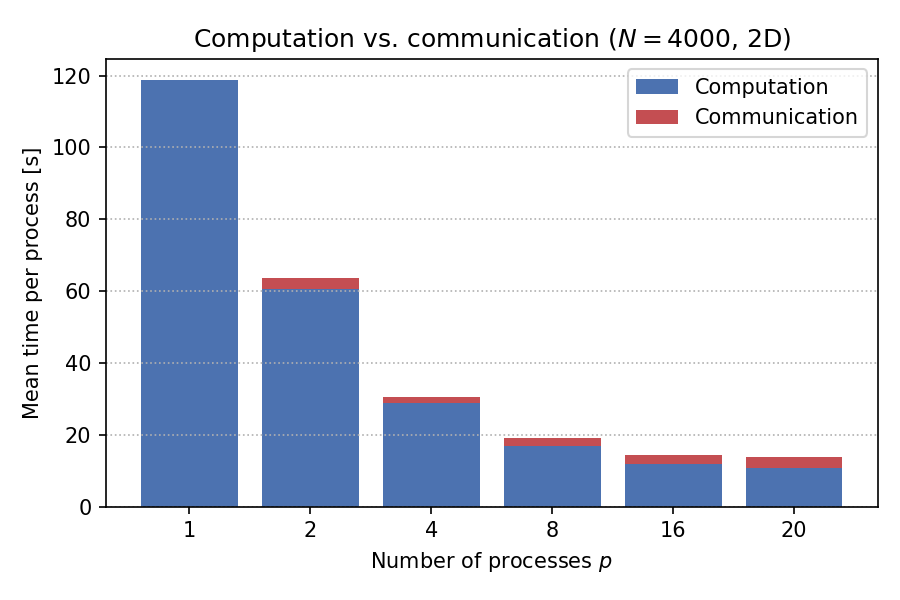
\includegraphics[width=0.6\textwidth]{figures/comm_compute.png}
\caption{Stacked computation vs.\ communication time per process ($N=2000$, 2D).}
\label{fig:commcompute}
\end{figure}

\subsection{Scalability}
Finally, we assess weak scaling by keeping the workload per process fixed at approximately $500 \times 500$ cells and increasing both the grid size and the process count together ($N = 500\sqrt{p}$). Ideal weak scaling would keep the total runtime constant. Figure~\ref{fig:weak} shows that the \emph{computation} time is indeed almost flat (it stays in the $0.64$--$0.85$~s band across $p = 1 \to 16$), which validates the load balancing of the decomposition. The \emph{total} runtime, however, drifts upward: it doubles from $p=1$ ($0.64$~s) to $p=4$ ($0.80$~s, weak efficiency $0.80$), and then degrades sharply for $p = 9$ and $p = 16$. The latter two points require \emph{oversubscribing} the 8 physical cores, so their inflation is a hardware artifact rather than an algorithmic one, and it is again driven by the communication term.

\begin{table}[h]
\centering
\caption{Weak scaling (2D, $\approx 500\times500$ cells/process). Points $p=9,16$ oversubscribe the 8 cores.}
\label{tab:weak}
\begin{tabular}{lcccc}
\toprule
$p$ (grid $N$) & 1 (500) & 4 (1000) & 9 (1500) & 16 (2000) \\
\midrule
Total time [s]   & 0.639 & 0.800 & 1.660 & 3.481 \\
Compute time [s] & 0.636 & 0.640 & 0.793 & 0.849 \\
Weak efficiency  & 1.00 & 0.80 & 0.39 & 0.18 \\
\bottomrule
\end{tabular}
\end{table}

\begin{figure}[h]
\centering
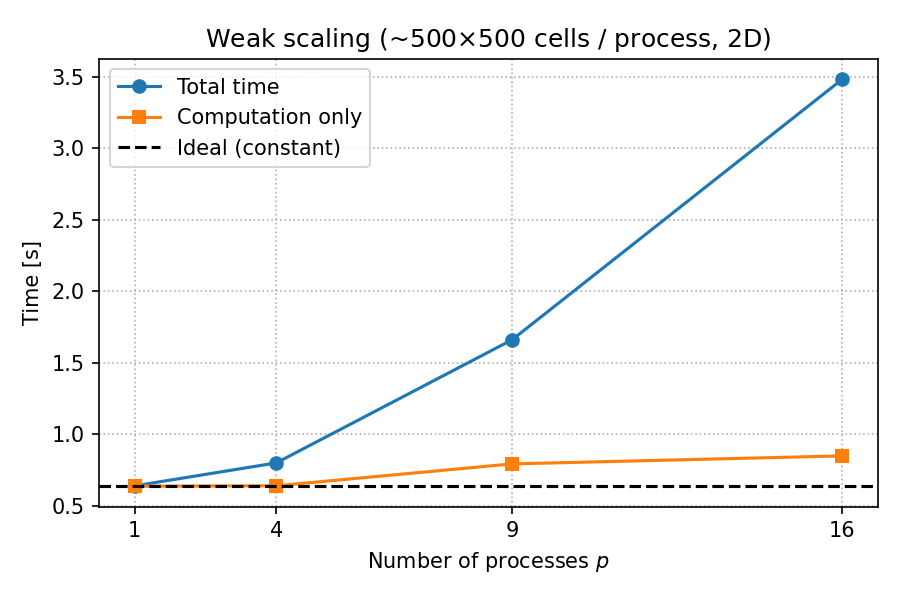
\includegraphics[width=0.6\textwidth]{figures/weak_scaling.png}
\caption{Weak scaling: total and computation-only time per process.}
\label{fig:weak}
\end{figure}

\section{Discussion}
Interpret the results, do not just describe them.

\subsection{Limitations}
Honest assessment: what the experiments do not show, what would need a multi-node cluster, what artifacts may arise from running all topologies on a single machine, ecc.

\subsection{Possible improvements}
Concrete next steps (es. uso di comunicazioni non bloccanti \texttt{MPI\_Isend} / \texttt{MPI\_Irecv} per sovrapporre calcolo e comunicazione in modo asincrono).


\section{Conclusions}
5-10 sentences. The headline result and the main lesson learned.

\begin{thebibliography}{1}
\bibitem{cormen}
T. H. Cormen, C. E. Leiserson, R. L. Rivest, C. Stein, \textit{Introduction to Algorithms}, 4th ed., MIT Press.
\bibitem{mpi4py}
L. Dalcin, \textit{mpi4py: MPI for Python}, Journal of Parallel and Distributed Computing.
\bibitem{drossel1992}
B. Drossel, F. Schwabl, \textit{Self-organized critical forest-fire model}, Physical Review Letters, 69(11), 1629, 1992.
\end{thebibliography}

\end{document}